\documentclass[9pt,landscape]{article}

\usepackage{multicol}
\usepackage{amsmath}

\usepackage{amssymb}
\usepackage{amsthm}
\usepackage{amsmath}
\usepackage{fontspec,xunicode,xltxtra}
\usepackage{titlesec}
\usepackage{indentfirst}
\usepackage{xeCJK}
\usepackage{fancyhdr}
\usepackage{graphicx}
\usepackage{listings}
\usepackage{printlen}
\usepackage{ifthen}
\usepackage[savepos]{zref}
\usepackage{multicol}
\usepackage{sectsty}
\usepackage{xcolor}
\usepackage[framemethod=tikz]{mdframed}
\usepackage{hyperref}

\usepackage[paper=a4paper]{geometry}
\geometry{headheight=2.6cm,headsep=3mm,footskip=13mm}
\geometry{top=2cm,bottom=2cm,left=2cm,right=2cm}


\setCJKmainfont[BoldFont={SimHei}]{SimSun}
\newfontfamily{\monotype}{Consolas}
%\newcommand{\monotype}{\tt}

\pagestyle{fancy}

\fancyhead[L]{重生之我带着记忆回到 MH3511 考前}
\fancyhead[C]{今晚必是不眠之夜}
\fancyhead[R]{但我们已无路可退——身后就是莫斯科!}

\setlength{\parindent}{0em}

% settings for listings
\lstset {
  basicstyle = \small\monotype,
  language = R,
  tabsize = 2,
  breaklines = true,
  breakindent = 1.1em,
%  numbers=right,
  aboveskip=2pt,  % 设置代码框上方的间距
  belowskip=2pt,  % 设置代码框下方的间距
  stringstyle=\monotype,
  numberstyle=\footnotesize\ttfamily,
  firstnumber=last,
  basewidth={0.5em, 0.4em},
  frame=single
}

\usepackage{titlesec}

% Adjust spacing for section
\titlespacing*{\section}{0pt}{1ex plus 0.5ex minus .2ex}{1ex plus .2ex}

% Adjust spacing for subsection
\titlespacing*{\subsection}{0pt}{1ex plus 0.5ex minus .2ex}{1ex plus .2ex}

% Adjust spacing for subsubsection
\titlespacing*{\subsubsection}{0pt}{1ex plus 0.5ex minus .2ex}{1ex plus .2ex}

\usepackage{enumitem}
\setlist[enumerate]{itemsep=0pt, parsep=0pt, topsep=0pt}

% an amazing script
% converts an line-number to arbitrary string
\let\othelstnumber=\thelstnumber
\def\createlinenumber#1#2{
    \edef\thelstnumber{%
        \unexpanded{%
            \ifnum#1=\value{lstnumber}\relax
             \tt #2%
            \else}%
        \expandafter\unexpanded\expandafter{\thelstnumber\othelstnumber\fi}%
    }
    \ifx\othelstnumber=\relax\else
      \let\othelstnumber\relax
    \fi
}

\usepackage{enumitem}

\setlist[itemize]{itemsep=0pt}
 % formatting template

\begin{document}

\begin{multicols}{3}

\columnseprule=0.25pt

\section{常用代码及公式}

$\frac{1}{\sigma^2}\sum(X_i-\mu)\sim\chi^2_n$

$\frac{1}{\sigma^2}\sum(X_i-\overline{X})\sim\chi^2_{n-1}$

$\frac{\overline{X}-\mu}{S/\sqrt{n}}\sim t_{n-1}$ ($n\ge 30$ 当 $\mathcal{N}$)

\texttt{qnorm}: 生成 normal 数据

\section{Measurement}

\textbf{Scales of Measurement}

\begin{enumerate}
	\item nominal: 没有 order 的 categories
	\item ordinal: 有 order
	\item interval: 数值按照等长区间分类
	\item ratio: 单点的数值
\end{enumerate}

\textbf{数据的分类}
\begin{enumerate}
	\item Categorical / Qualitative: Nominal / Ordinal
	\item Numerical / Quantitative: Discrete / Continuous
\end{enumerate}

\textbf{Basic Quantities}

\texttt{quantile(arr, 0.25)}: $Q_1$

$Q_{1, 2, 3}$: $25\%$, $50\%$, $75\%$ percentile

$\mathrm{IQR}=Q_3-Q_1$

Skewness: 看尾巴在哪边
\begin{enumerate}
	\item Left-Skewed: Negative Skewness
	\item Right-Skewed: Positive Skewness
\end{enumerate}

\textbf{Why trimmed mean?}
\begin{enumerate}
	\item May have a lower SE when data is not normal
	\item Balance between median and mean, protect against outliers
\end{enumerate}

\textbf{画图}
\begin{enumerate}
	\item Stem and leaf plot: 左边是数字第一位,右边是后面的,中间用 \texttt{|} 隔开(\texttt{stem(x)})
	\item Histogram: \texttt{hist(x)}
\end{enumerate}

\textbf{transformation}

log 把中心往右,exp 把中心往左

Log-normal distribution: $\log X\sim\mathcal{N}(\mu,\sigma^2)$

$f(x)=\frac{1}{x\sigma\sqrt{2\pi}}e^{-\frac{(\log x-\mu)}{2\sigma^2}}$

$\mu=e^{\mu+\frac{\sigma^2}{2}}$, $\sigma^2=[\exp(\sigma^2)-1]\exp(2\mu+\sigma^2)$

\textbf{Coefficient of Variation (CV)}: $\frac{\sigma}{\mu}$

$\mathrm{Geomean}=\sqrt[n]{\prod X_i}$

\textbf{Imposing a Normal PDF on the Histogram}

\begin{lstlisting}
	hist(x)
	xpt <- seq(from, to, by=by)
	n_den <- dnorm(xpt, mean(return), sd(return))
	ypt <- n_den * length(x) * 10
	# We notice that each data point in the return dataset represents an area of 1 * 10, so the total area of the histogram would be * 10. 
	lines(xpt, ypt, col="blue")
\end{lstlisting}

\textbf{QQplot}: $\left(\Phi^{-1}(q_i), \hat{F}^{-1}_x(q_i)\right)$
\begin{enumerate}
	\item 左侧越低表示 longer left tail
	\item 右侧越高表示 longer right tail
\end{enumerate}

left skew 是两侧都高,right skew 是两侧都低

t 两个尾巴都长,是左低右高

\textbf{Shapiro-Wilk Test}: \texttt{shapiro.test(x)}

$W=\frac{\left(\sum_{i=1}^{n}a_ix_i\right)^2}{\sum_{i=1}^{n}(x_i-\overline{x})^2}$,$a_i$ 是这个系统自带的常数

$p$ 越小越 normal

Limitations:
\begin{enumerate}
	\item Adversely affected when there are tied data
	\item Has a bias by sample size. Statistically significant result, large sample.
\end{enumerate}

\textbf{box-plot}: \texttt{boxplot(x\textasciitilde group, data=x)}

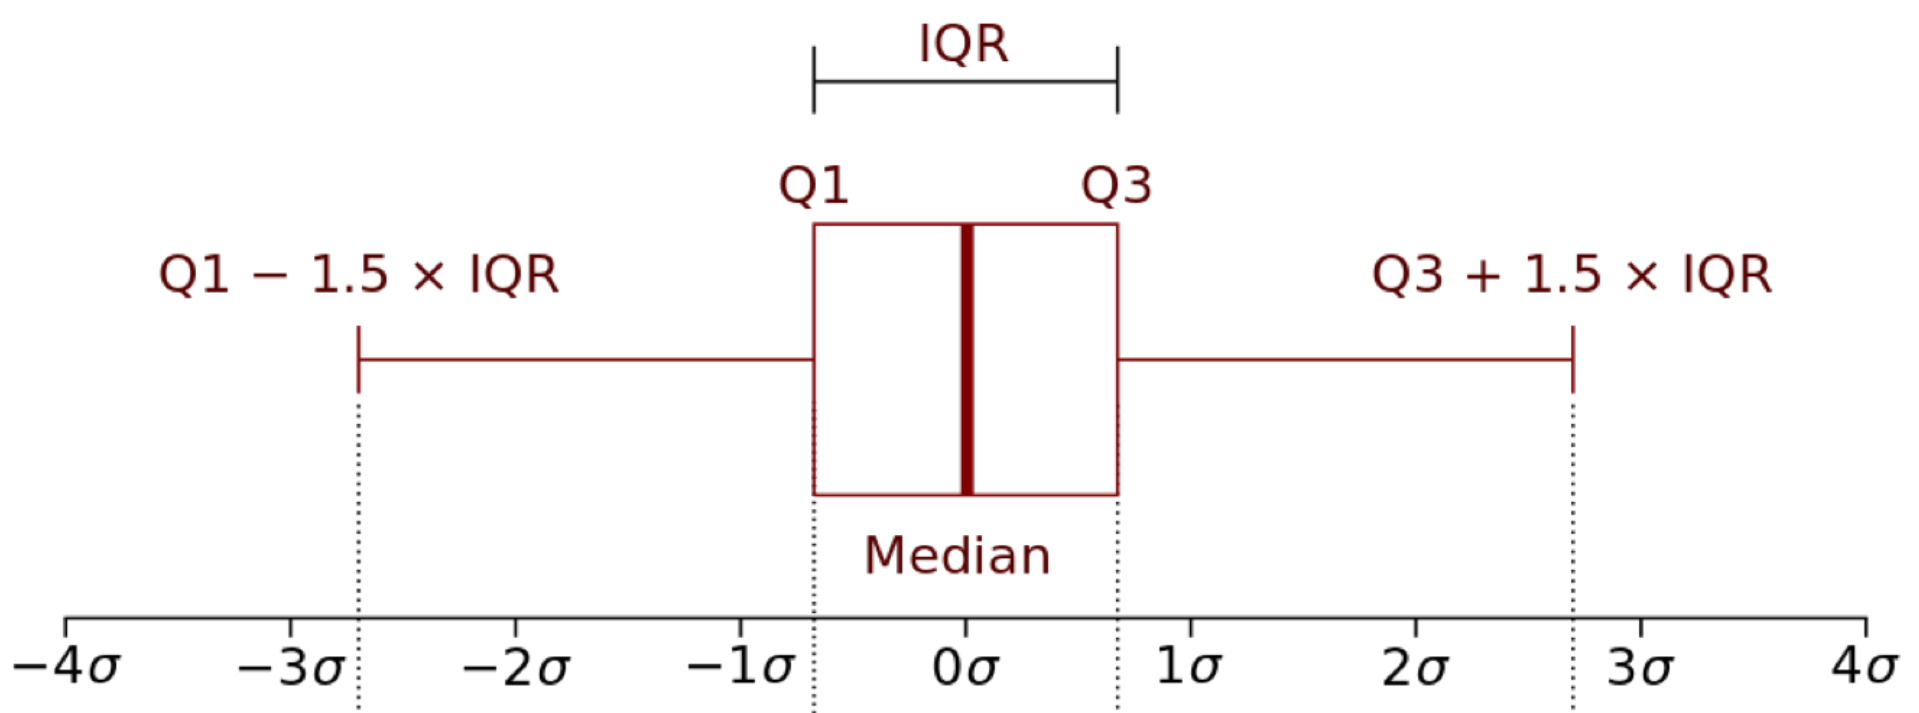
\includegraphics[width=0.7\columnwidth]{imgs/boxplot}

\textbf{Outliers}

classic tech: $|x_i-\overline{x}|>2\cdot\mathrm{sd}$

boxplot rule: $x_i<Q_1-1.5\cdot\mathrm{IQR}$ or $x_i > Q_3+1.5\cdot\mathrm{IQR}$

\end{multicols}

\end{document}
